\begin{frame}{Montagens e componentes medidos}
  \small
  \begin{columns}[T,onlytextwidth]
    \begin{column}{0.31\textwidth}
      \centering
      \textbf{Circuito 1}

      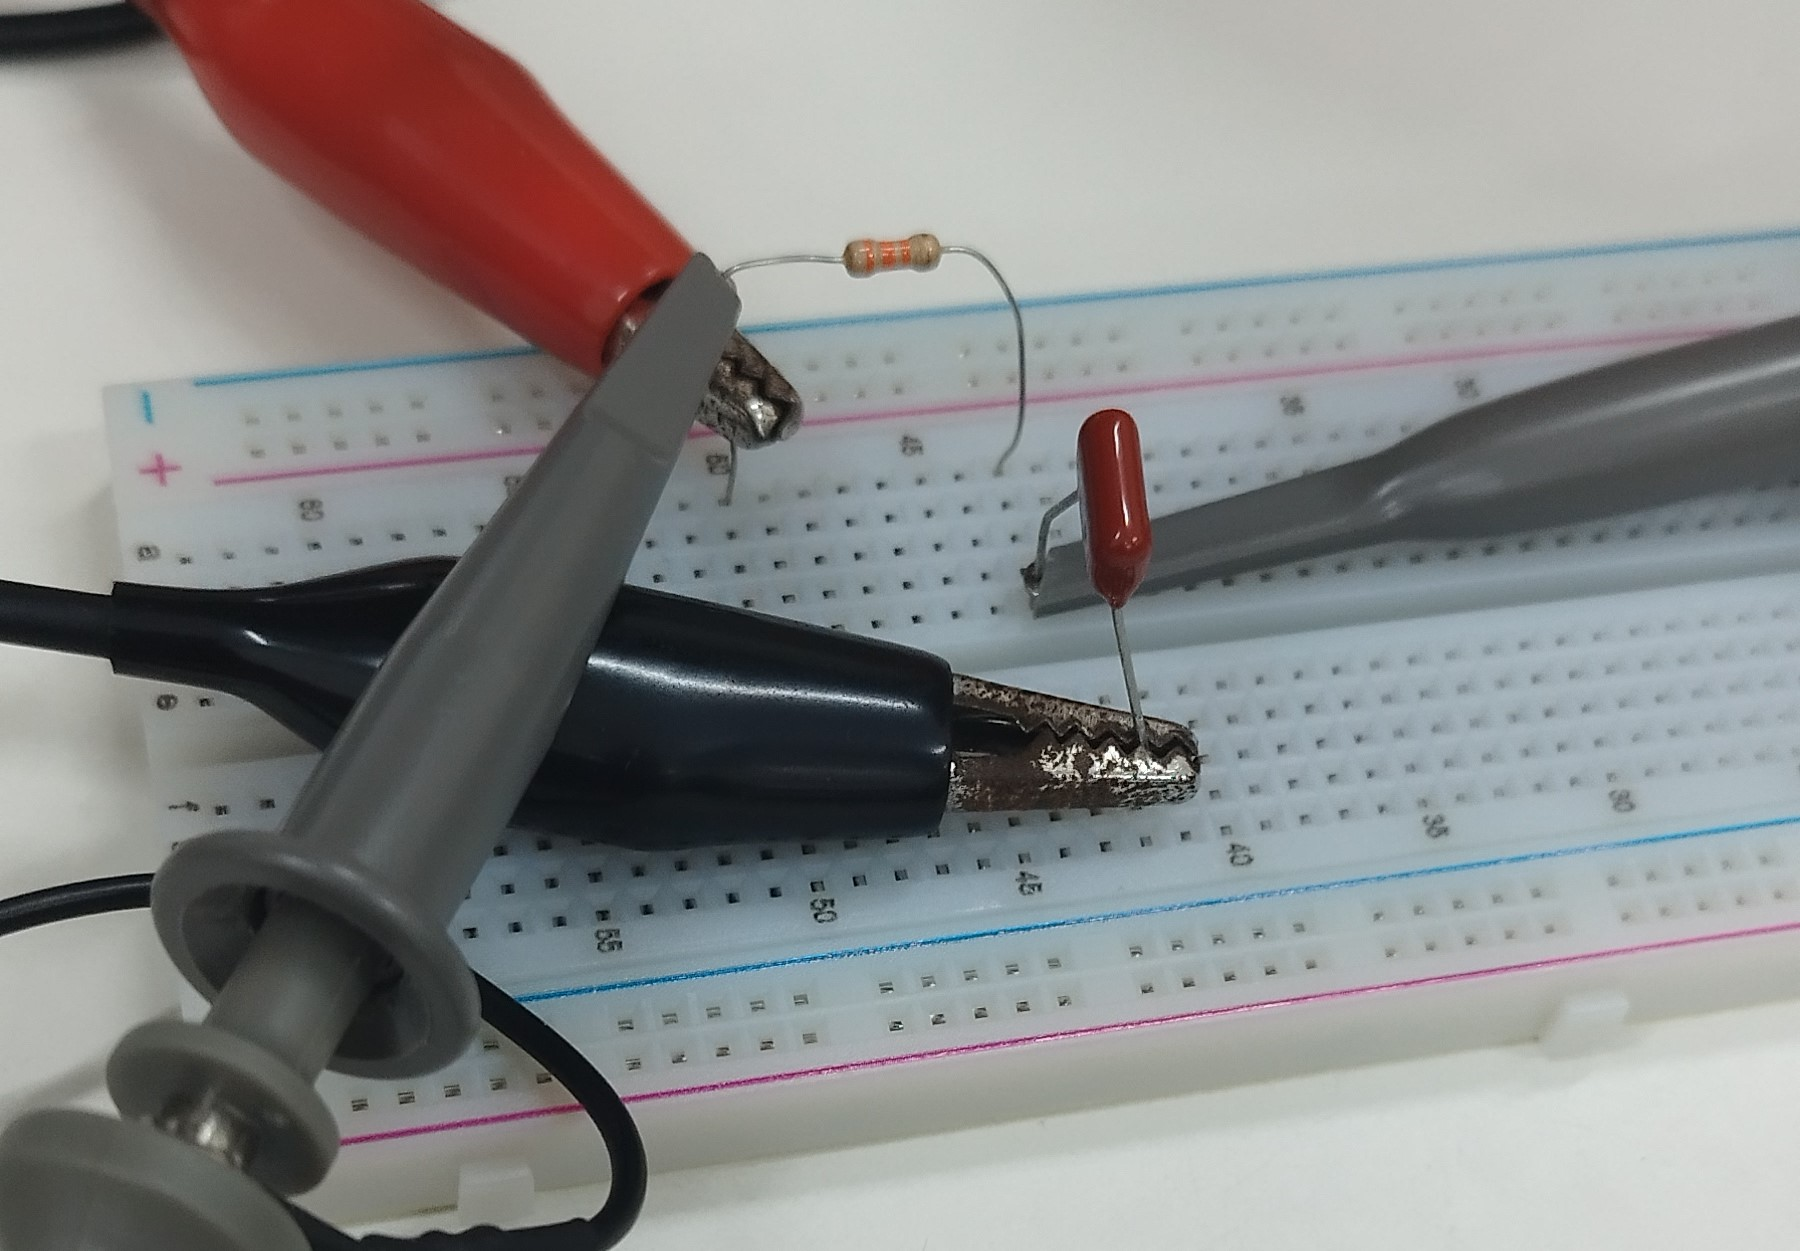
\includegraphics[width=\linewidth,height=0.24\textheight,keepaspectratio]{slides/img/protoboard_1.jpg}
    \end{column}
    \begin{column}{0.31\textwidth}
      \centering
      \textbf{Circuito 2}

      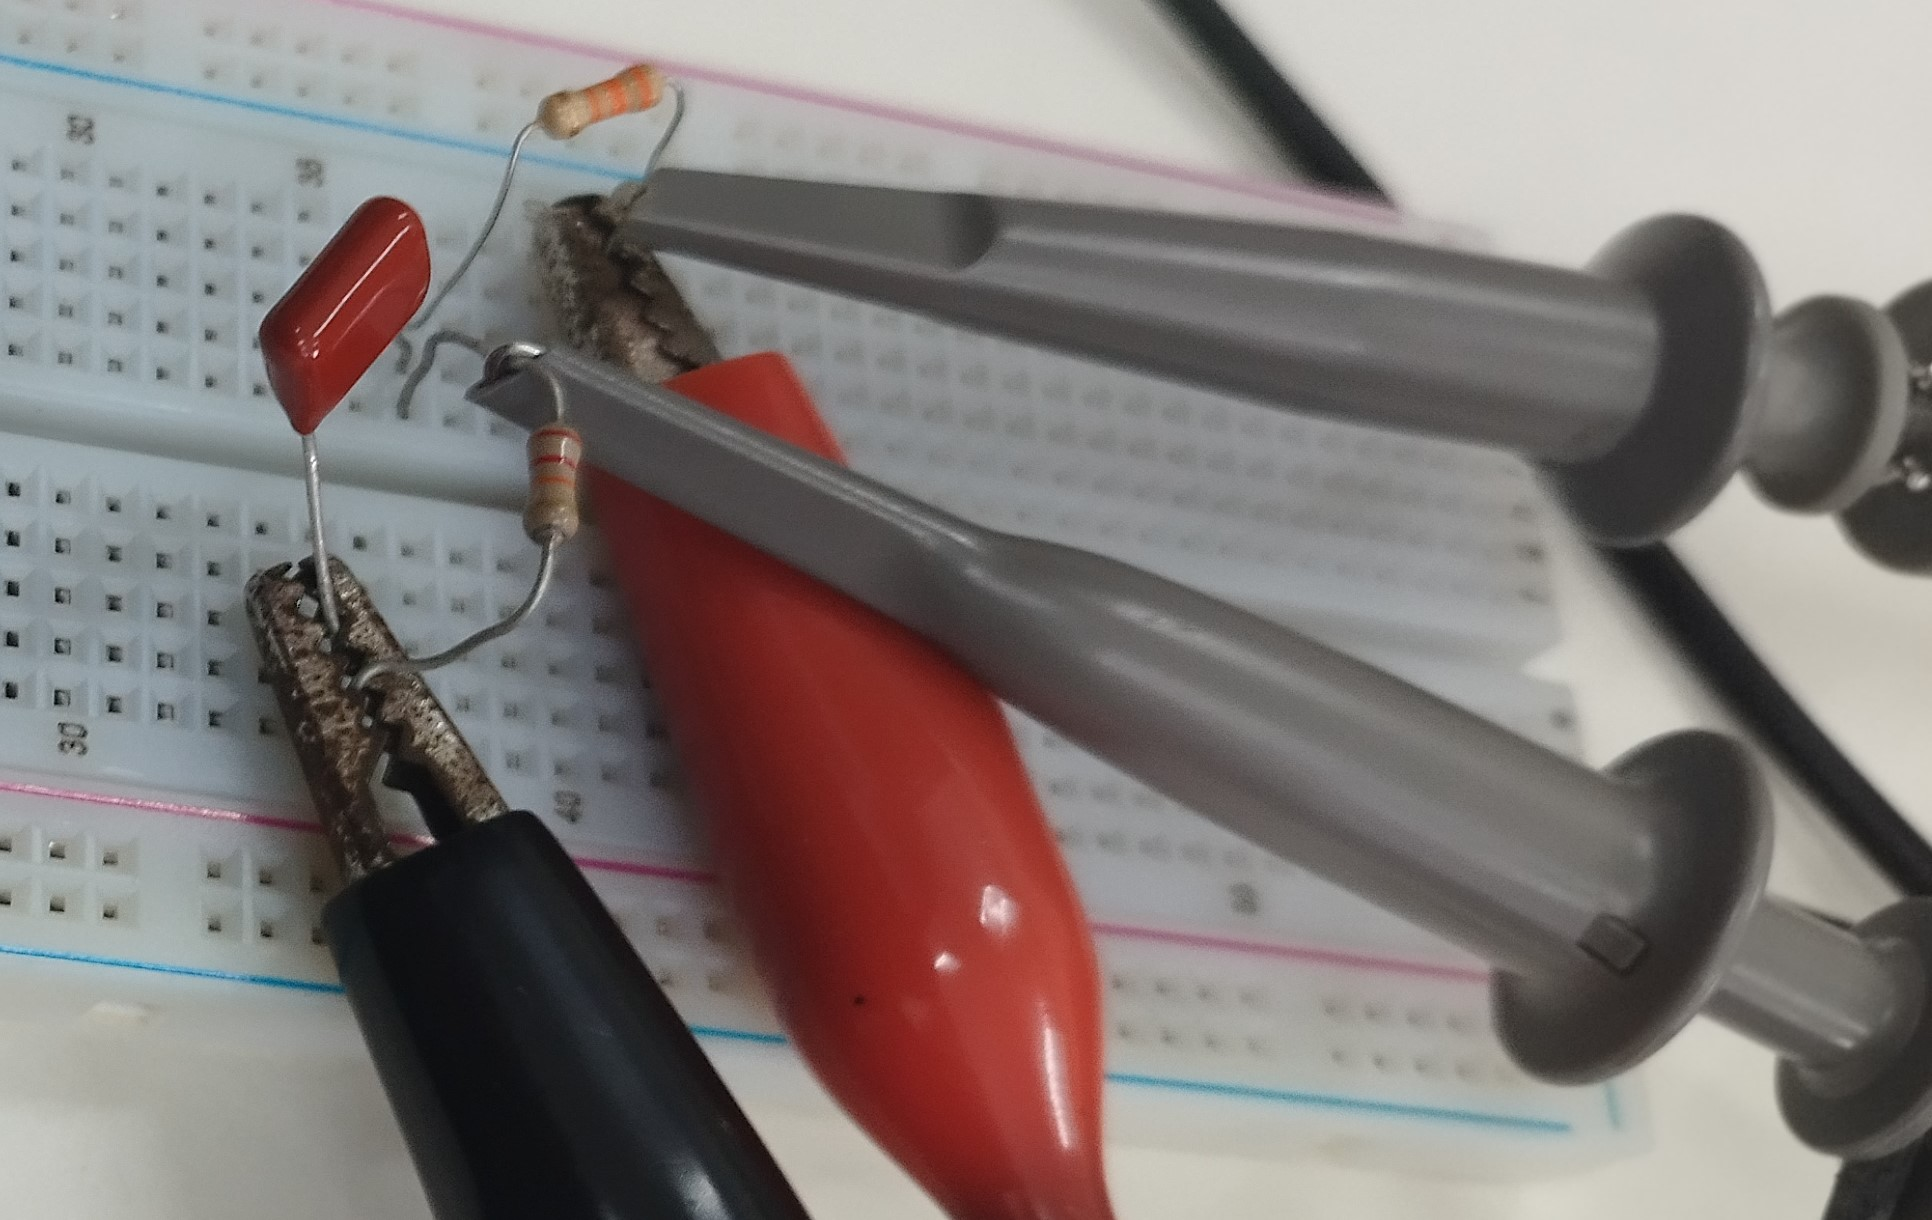
\includegraphics[width=\linewidth,height=0.24\textheight,keepaspectratio]{slides/img/protoboard_2.jpg}
    \end{column}
    \begin{column}{0.31\textwidth}
      \centering
      \textbf{Circuito 3}

      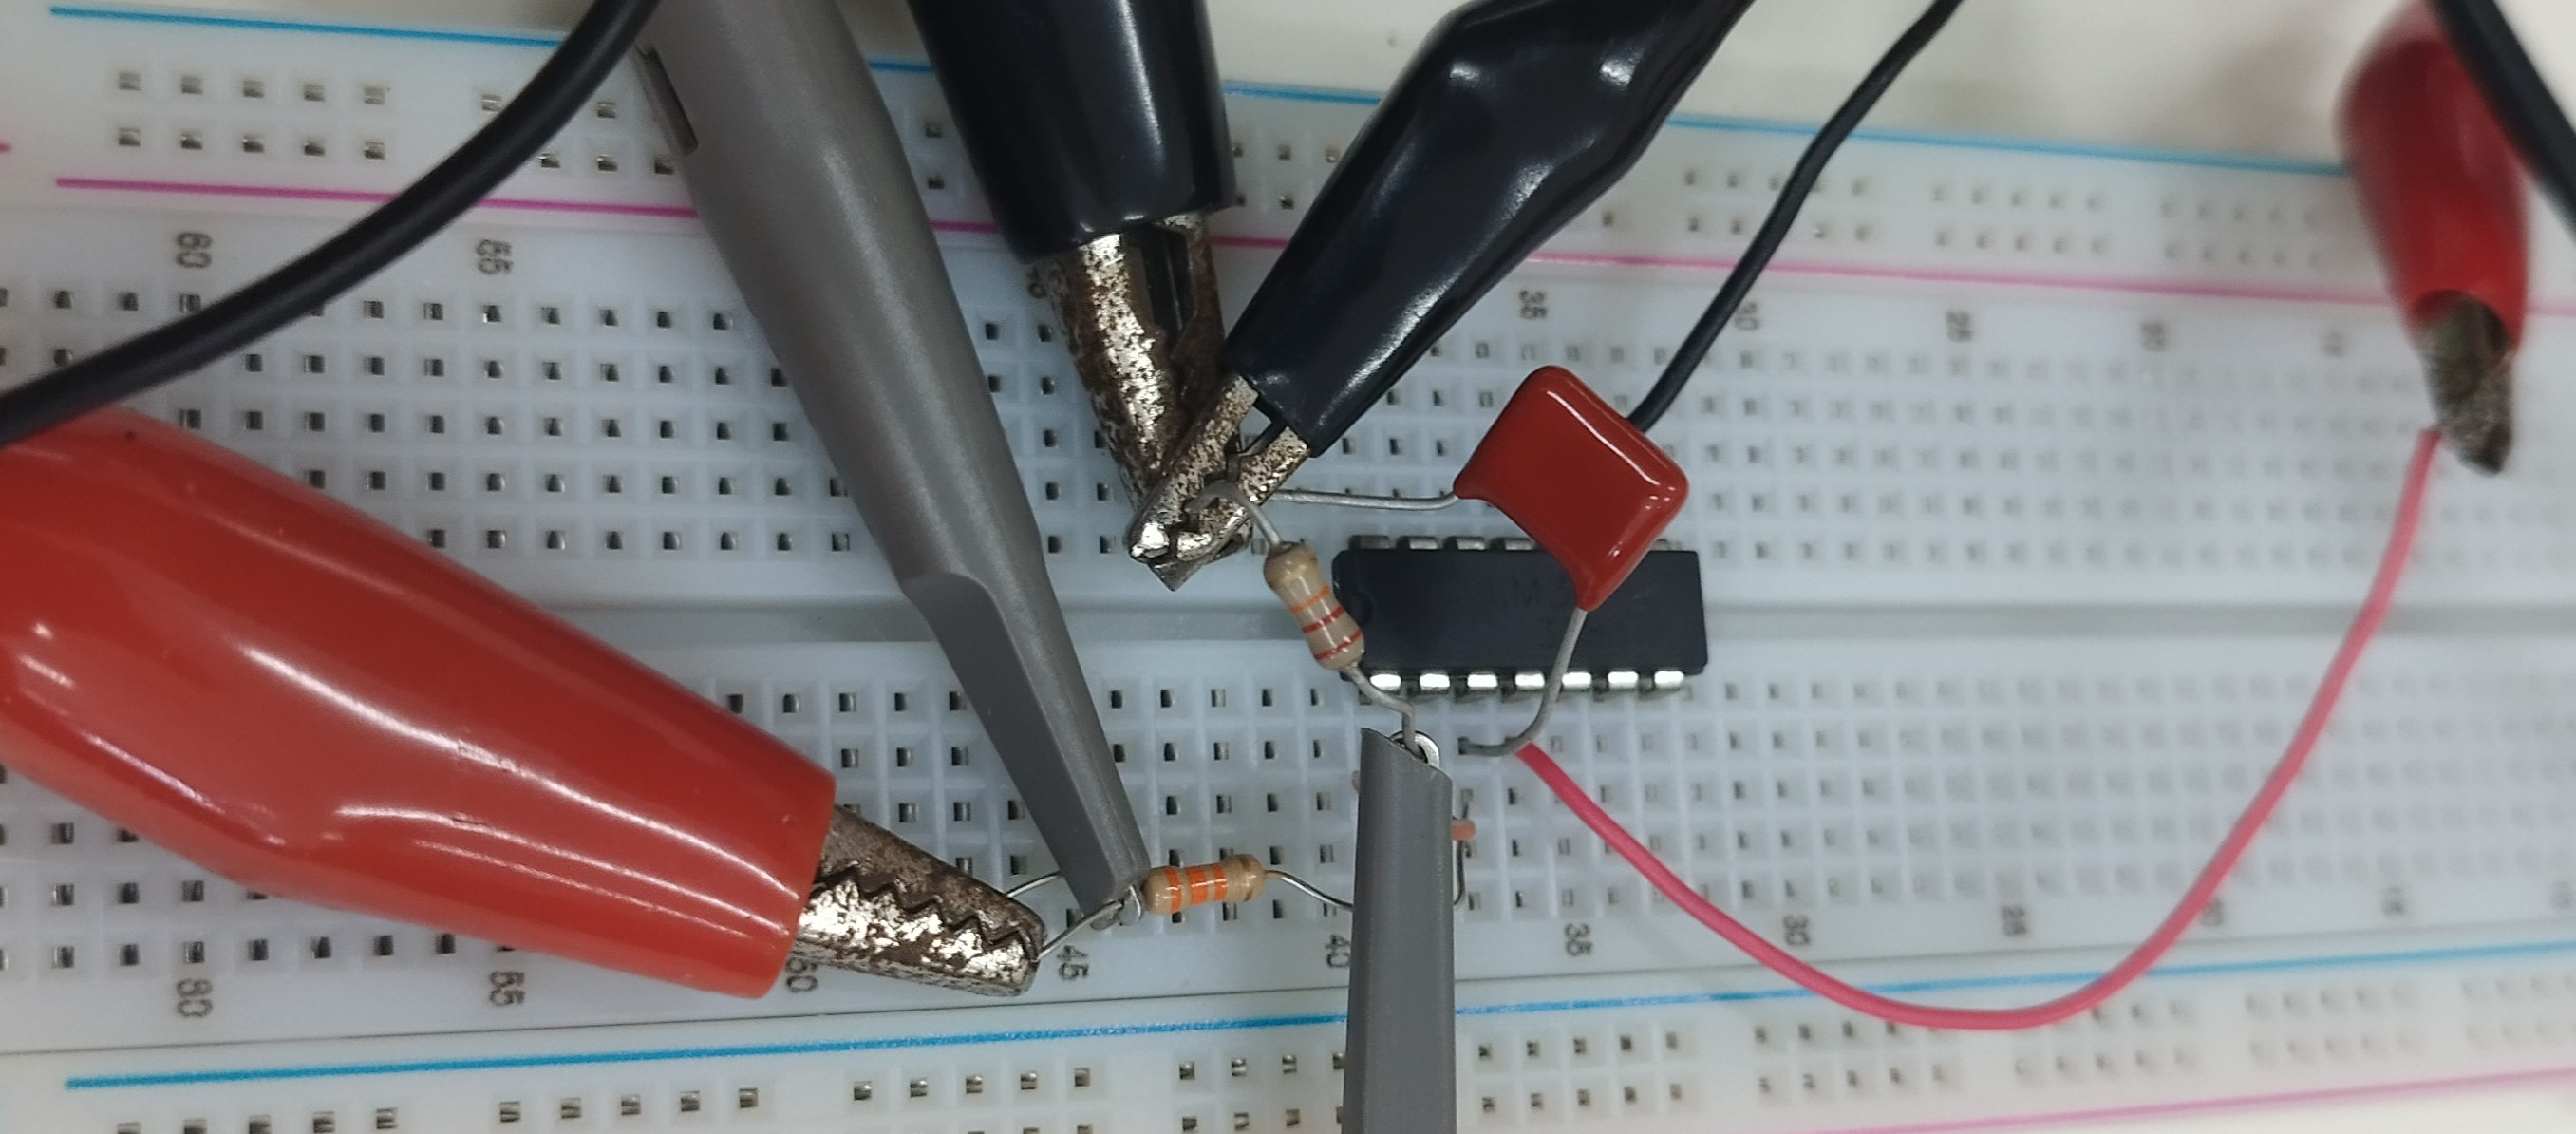
\includegraphics[width=\linewidth,height=0.24\textheight,keepaspectratio]{slides/img/protoboard_3.jpg}
    \end{column}
  \end{columns}

  \vspace{0.14cm}
  {\centering
    \renewcommand{\arraystretch}{1.0}
    \begin{tabular}{lccc}
      \toprule
      Circuito & $R$ ($\mathrm{k}\Omega$) & $C$ (nF) & $R_L$ ($\mathrm{k}\Omega$) \\
      \midrule
      1 -- sem carga & $21{,}841$ & $103{,}80$ & -- \\
      2 -- carga direta & $22{,}021$ & $110{,}90$ & $32{,}314$ \\
      3 -- buffer & $21{,}757$ & $106{,}28$ & $32{,}657$ \\
      \bottomrule
    \end{tabular}\par
  }

  \begin{alertblock}{Parâmetros da bancada}
    O conjunto medido difere do projeto de $50\,\mathrm{Hz}$.
    Cada modelo pós-laboratorial usa os componentes da respectiva montagem.
  \end{alertblock}
  \centering\scriptsize Registros de montagem das topologias; valores medidos usados nas comparações quantitativas.
\end{frame}
